% Created 2015-03-19 Thu 18:25
\documentclass[11pt]{article}
\usepackage[utf8]{inputenc}
\usepackage{lmodern}
\usepackage[T1]{fontenc}
\usepackage{fixltx2e}
\usepackage{graphicx}
\usepackage{longtable}
\usepackage{float}
\usepackage{wrapfig}
\usepackage{rotating}
\usepackage[normalem]{ulem}
\usepackage{amsmath}
\usepackage{textcomp}
\usepackage{marvosym}
\usepackage{wasysym}
\usepackage{amssymb}
\usepackage{amsmath}
\usepackage[version=3]{mhchem}
\usepackage[numbers,super,sort&compress]{natbib}
\usepackage{natmove}
\usepackage{url}
\usepackage{minted}
\usepackage{underscore}
\usepackage[linktocpage,pdfstartview=FitH,colorlinks,
linkcolor=blue,anchorcolor=blue,
citecolor=blue,filecolor=blue,menucolor=blue,urlcolor=blue]{hyperref}
\usepackage{attachfile}
\usepackage[left=1in, right=1in, top=1in, bottom=1in, nohead]{geometry}
\usepackage{fancyhdr}
\usepackage{hyperref}
\usepackage{setspace}
\usepackage[labelfont=bf]{caption}
\usepackage{amsmath}
\usepackage{enumerate}
\usepackage[parfill]{parskip}
\date{Due: 02/12/2015}
\title{}
\begin{document}

\title{Homework 3\\Lectures 4: Electronic Structure Models\\(CBE 60547)}
\author{Prateek Mehta, Prof. William F.\ Schneider}
\maketitle


Here is an example input deck for a HFS/6-31G calculation on NH$_{\text{3}}$. This is a good starting template for the calculations below. You can also construct an input deck in Avogadro. Refer to the GAMESS manual for more information.

\begin{verbatim}
!   File created by the GAMESS Input Deck Generator Plugin for Avogadro
 $BASIS GBASIS=N31 NGAUSS=6 $END
 $CONTRL RUNTYP=ENERGY DFTTYP=SLATER $END

 $DATA 
Title
C1
N     7.0    -1.03363     0.80618     0.00000
H     1.0    -0.01363     0.80618     0.00000
H     1.0    -1.37362     1.64340    -0.47314
H     1.0    -1.37363     0.79732     0.96162
 $END
\end{verbatim}


\section{\texttt{GAMESS} vs. \texttt{FDA}}
\label{sec-1}

Using \texttt{GAMESS}, perform a DFT/Hartree-Fock-Slater (\verb~DFTTYP=SLATER~) calculation on an Ar atom using the 6-31G basis set.

\begin{enumerate}[(a)]
\item How many primitive Gaussians are included in this calculation? How many total basis functions? How do they divide between s, p, and d?

\item How many SCF iterations does the calculation take to converge?

\item What is the final calculated HFS/6-31G energy of the atom?

\item What are the identities (1s, 2p, etc.) and energies of the occupied atomic orbitals?

\item Compare your computed total energy and atomic orbital energies with those you got from Homework 2 using the fda code for Ar.
\end{enumerate}


\subsection{Solution}
\label{sec-1-1}

\subsubsection{a)}
\label{sec-1-1-1}

This is an example input file for Ar. The resulting output files can be seen in ./Ar

\begin{verbatim}
 $BASIS GBASIS=N31 NGAUSS=6 $END
 $CONTRL RUNTYP=ENERGY DFTTYP=SLATER $END

 $DATA 
Title
C1
Ar    18.0    -3.86612     1.03789     0.00000
 $END
\end{verbatim}

By looking at the log file it seems we have 13 primitive Gaussians. Below is the shell command to produce this result.

\begin{minted}[frame=lines,fontsize=\scriptsize,linenos]{sh}
grep "GAUSSIAN BASIS FUNCTIONS" Ar/Ar.log
\end{minted}

\begin{verbatim}
NUMBER OF CARTESIAN GAUSSIAN BASIS FUNCTIONS =   13
\end{verbatim}

We used the 6-31G basis set. The distribution of basis functions are listed below.

\begin{center}
\begin{tabular}{lrrr}
Orbital & Basis Sets & Primitive gauss functions & Total gauss functions\\
\hline
1s & 1 & 6 & 6\\
2s & 1 & 6 & 6\\
2p & 3 & 6 & 18\\
3s & 1 & 3 & 3\\
3p & 3 & 3 & 9\\
3s+ & 1 & 1 & 1\\
3p+ & 3 & 1 & 3\\
\hline
Total & 13 &  & 46\\
\end{tabular}
\end{center}



\subsubsection{b)}
\label{sec-1-1-2}

12 SCF iterations are required to reach convergence.

\begin{minted}[frame=lines,fontsize=\scriptsize,linenos]{sh}
grep "ITER" Ar/Ar.dat
\end{minted}

\begin{verbatim}
E(R-SLATER)=     -524.4520526614, E(NUC)=    0.0000000000,   12 ITERS
\end{verbatim}


\subsubsection{c)}
\label{sec-1-1-3}

The final HFS/6-31G energy is -524.452  hartrees.

\subsubsection{d)}
\label{sec-1-1-4}

\begin{table}[htb]
\caption{\texttt{GAMESS} and \texttt{FDA} orbital energies \label{orbital-energies}}
\centering
\begin{tabular}{lrr}
Orbital & E$_{\text{GAMESS}}$ (hartree) & E$_{\text{FDA}}$ (hartree)\\
\hline
1s & -113.6768 & -116.9366\\
2s & -10.7172 & -11.6037\\
2p & -8.3677 & -9.2721\\
3s & -0.8218 & -1.1022\\
3p & -0.3222 & -0.5735\\
3s+ & 0.4316 & \\
3p+ & 0.5206 & \\
\end{tabular}
\end{table}


\subsubsection{e)}
\label{sec-1-1-5}

The \texttt{FDA} total energy is -526.8275 hartree, which means its a slightly better method for predicting the energy of Ar. The orbital energies are listed in table \ref{orbital-energies}. 

\section{The Generalized Gradient Approximation}
\label{sec-2}

The generalized gradient approximation (GGA) is an improvement on Hartree-Fock-Slater that gives a nice balance between accuracy and computational expense. Using \texttt{GAMESS}, perform a single point calculation (\verb~RUNTYP=ENERGY~) on the bent triatomic SO$_{\text{2}}$ using the GGA (\verb~DFTTYP=PBE~) and PC1 basis set (\verb~GBASIS=PC1~, \verb~ISPHER=1~; no \verb~NGAUSS~ flag needed). Guess appropriate bond lengths and angle. Be sure to report your input file for your calculation.

\begin{enumerate}[(a)]
\item What is the spin multiplicity of SO$_{\text{2}}$? (Recall, the spin multiplicity is 2S +1, where S = 1/2 for one unpaired electron, S = 1 for two unpaired electrons, and so on).

\item How many basis functions are in this calculation?

\item How many SCF cycles does it take to converge?

\item What SCF algorithm does the code use?

\item What is the final total energy of the molecule?

\item How many occupied orbitals does the molecule have? What are the energies of the HOMO and LUMO?

\item What is the final dipole moment?

\item What are the Mulliken gross charges on the S and O atoms?

\item Plot out the electrostatic potential of SO$_{\text{2}}$. Which end of the molecule is electrophilic and which is nucleophilic?
\end{enumerate}

\subsection{Solution}
\label{sec-2-1}

The relevant files can be found at the github repository for the course.

INPUT File: \url{./SO2/SO2.inp}

LOG File: \url{./SO2/SO2.log}

DAT File: \url{./SO2/SO2.dat}

\subsubsection{a)}
\label{sec-2-1-1}

The spin multiplicity for SO$_{\text{2}}$ is 2 * 0 + 1 = 1. 

\subsubsection{b)}
\label{sec-2-1-2}
The number of basis functions in the calculation is 49.

\begin{minted}[frame=lines,fontsize=\scriptsize,linenos]{sh}
grep "GAUSSIAN BASIS FUNCTIONS" ./SO2/SO2.log
\end{minted}

\begin{verbatim}
NUMBER OF CARTESIAN GAUSSIAN BASIS FUNCTIONS =   49
\end{verbatim}


\subsubsection{c)}
\label{sec-2-1-3}

It takes 23 SCF cycles to converge.

\begin{minted}[frame=lines,fontsize=\scriptsize,linenos]{sh}
grep "ITER" ./SO2/SO2.dat
\end{minted}

\begin{verbatim}
E(R-PBE)=     -548.2499367382, E(NUC)=  109.8468077125,   23 ITERS
\end{verbatim}

\subsubsection{d)}
\label{sec-2-1-4}

The code uses the DIIS algorithm.


\subsubsection{e)}
\label{sec-2-1-5}

The final total energy is -548.2499 hartrees

\subsubsection{f)}
\label{sec-2-1-6}

There are 16 occupied orbitals.

\begin{minted}[frame=lines,fontsize=\scriptsize,linenos]{sh}
grep "OCCUPIED" ./SO2/SO2.log
\end{minted}

\begin{verbatim}
NUMBER OF OCCUPIED ORBITALS (ALPHA)          =   16
NUMBER OF OCCUPIED ORBITALS (BETA )          =   16
   16 ORBITALS ARE OCCUPIED (    7 CORE ORBITALS).
\end{verbatim}




\subsubsection{g)}
\label{sec-2-1-7}

The final dipole moment is 1.55 debyes

\subsubsection{h)}
\label{sec-2-1-8}

The Mulliken charges are tabulated below.

\begin{center}
\begin{tabular}{lr}
ATOM & CHARGE\\
\hline
S & 0.768910\\
O & -0.393816\\
O & -0.375094\\
\end{tabular}
\end{center}


\subsubsection{i)}
\label{sec-2-1-9}

The electrostatic potential is shown below.

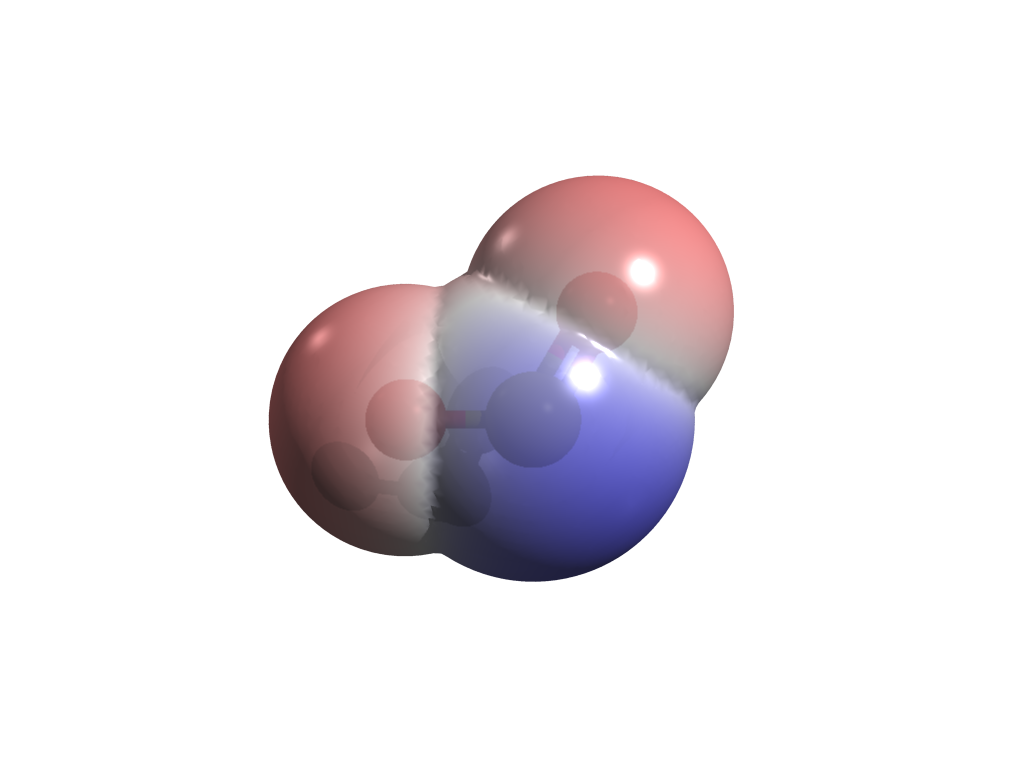
\includegraphics[width=.9\linewidth]{SO2/SO2-electrostatic-potential.png}

\section{Geometry Optimization of SO$_{\text{2}}$}
\label{sec-3}

\begin{enumerate}[(a)]
\item Do a series of calculations in which you vary the S–O distances and O–S–O angle over a regular grid of values. Approximate the combination of values that give the lowest energy.

\item A geometry optimization (\verb~RUNTYP=OPTIMIZE~) is a faster way to find the optimal geometry of a molecule. Perform a geometry optimization on SO$_{\text{2}}$ using the same computational model as above. What are the optimal S–O distances and O–S–O angle?
\end{enumerate}

\subsection{Solution}
\label{sec-3-1}

\subsubsection{a)}
\label{sec-3-1-1}


\begin{enumerate}
\item Creating input files and running \texttt{GAMESS}
\label{sec-3-1-1-1}

Here is some python code that creates and runs \texttt{GAMESS} calculations over a grid of distances and angles. Note that there are more efficient ways of doing these kind of calculations by using the CRC queueing system, which we will learn about in future classes.

\begin{minted}[frame=lines,fontsize=\scriptsize,linenos]{python}
import os
import numpy as np

# Input file template
gamess_script=''' $BASIS GBASIS=PC1 $END
 $CONTRL COORD=ZMT ISPHER=1 RUNTYP=ENERGY DFTTYP=PBE $END

 $DATA 
Title
Cnv 2

S    
O 1 {0:1.2f} 
O 1 {0:1.2f} 2 {1}
 $END'''

distances = np.linspace(1.3, 1.7, 5)
angles = np.linspace(90., 150., 7)

# Path to current directory
cwd = os.getcwd()

for distance in distances:
    for angle in angles:
        
        # Create calculation directory
        wd = './SO2/optimize/{0:1.2f}-A/{1:1.2f}-deg/'.format(distance, angle)
        if not os.path.exists(wd):
            os.makedirs(wd)

        # Change into calculation directory
        os.chdir(wd)
        # Create an input file
        with open('gamess.inp', 'w') as f:
            f.write(gamess_script.format(distance, angle))     
        # Run GAMESS   
        os.system('rungms gamess.inp > gamess.log')
        # Change back to current working directory
        os.chdir(cwd)
\end{minted}


\item Finding the optimum distance and angle
\label{sec-3-1-1-2}

Now we will read the .dat files for the total energies and plot them. This is similar to what we did in Lab1. 

\begin{minted}[frame=lines,fontsize=\scriptsize,linenos]{python}
import numpy as np
import matplotlib.pyplot as plt

distances = np.linspace(1.3, 1.7, 5)
angles = np.linspace(90., 150., 7)

plt.figure(figsize = (6,8))
for angle in angles:
    
    energies = []
    for distance in distances:
        
        # Create calculation directory
        filename = './SO2/optimize/{0:1.2f}-A/{1:1.2f}-deg/gamess.dat'.format(distance, angle)

        with open(filename, 'r') as f:
            for line in f.readlines():
                # We want lines like
                # E(R-PBE)=     -547.9256306493, E(NUC)=  130.1179768731,   20 ITERS
                if 'E(R-PBE)' in line:
                    # Strip out the commas
                    line = line.replace(',', "")
                    # Now extract the energy
                    energy = float(line.split()[1])
                    energies.append(energy)
                    # Break out of the loop as we got the energy
                    break
    plt.plot(distances, energies, 'o-', label = '{0:1.0f} deg'.format(angle))
plt.legend(loc='best')
plt.xlabel('Distance ($\AA$)')
plt.ylabel('Energy (hartree)')
plt.ticklabel_format(useOffset=False) # make the y-axis without offset
plt.tight_layout()
plt.savefig('SO2-optimization.png')
plt.show()
\end{minted}

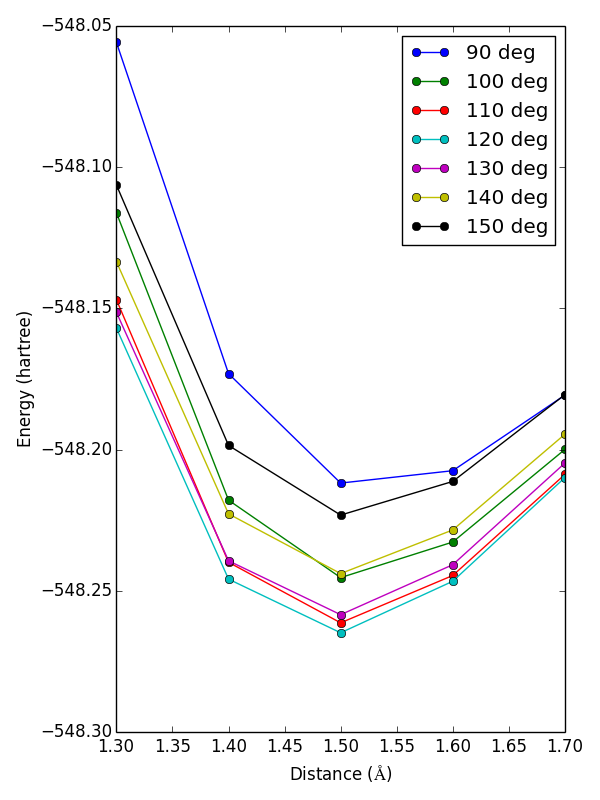
\includegraphics[width=3in]{./SO2-optimization.png}

From the plot it looks like the lowest energy is roughly around a O-S-O angle of 120\textdegree{} and O-S distance of 1.5 \AA{}. Note that we could have fit a curve to our data for a better approximation.
\end{enumerate}


\subsubsection{b)}
\label{sec-3-1-2}

Using \verb~RUNTYP=OPTIMIZE~ we have the S-O distance as 1.49 \AA{} and the O-S-O angle as 118.35\textdegree{}. Looks like we came pretty close using our rough scan!

LOG File: \url{SO2/SO2-opt.log}

\section{Other Molecules}
\label{sec-4}

Oxygen makes bonds with lots of things. Fill out the table below by doing an appropriate set of calculations:

\subsection{Solution}
\label{sec-4-1}
\begin{center}
\begin{tabular}{lrrrrl}
AO$_{\text{2}}$ & A-O (\AA{}) & O-A-O (\textdegree{}) & Spin Multiplicity & Dipole Moment (e\AA{}) & Mulliken Charge\\
\hline
CO$_{\text{2}}$ & 1.176 & 180 & 1 & 0 & C: 0.54, O: -0.27\\
NO$_{\text{2}}$ & 1.211 & 133.74 & 2 & 0.27 & N: 0.38, O: -0.19\\
SiO$_{\text{2}}$ & 1.538 & 180 & 1 & 0 & Si: 0.99, O: -0.50\\
SO$_{\text{2}}$ & 1.490 & 118.35 & 1 & 1.88 & S: 0.82, O: -0.41\\
\end{tabular}
\end{center}
% Emacs 24.4.3 (Org mode 8.2.10)
\end{document}